\section{Amplificatori Operazionali Ideali - 16.09.2014}

In questa prima sessione di laboratorio abbiamo preparato la breadboard con il circuito di alimentazione per l'amplificatore operazionale (opamp) che useremo anche nelle successive esperienze.
Una volta preparata l'alimentazione, abbiamo montato due circuiti con opamp e valutato il loro funzionamento misurando la loro tensione di output.

\subsection*{Strumenti e materiali}

\begin{itemize} [noitemsep]
\item Oscilloscopio Agilent DSO-X 2002A (bandwidth \SI{70}{\mega\hertz}, sample rate \num{2} GSa/s);
\item Generatore di tensione continua Agilent E3631A (max $\pm \, \SI{25}{\volt}$ o $\pm \, \SI{6}{\volt}$);
\item Generatore di forme d'onta Agilent 33120A con range di frequenza da \SI{100}{\micro\hertz} a \SI{15}{\mega\hertz};
\item Multimetro Agilent 34410A (utilizzato come amperometro e per verificare i valori delle resistenze);
\item Un amplificatore operazionale $\mu$A741;
\item Resistenze di vari valori;
\item Due capacità da \SI{100}{\nano\farad};
\item un trimmer (potenziometro);
\item Breadboard e cablaggi vari.
\end{itemize}

\subsection{Premessa sugli amplificatori operazionali ideali}

Nelle nostre esperienze tratteremo gli amplificatori operazionali considerandoli componenti ideali. Tale approssimazione non è limitante visti i valori di corrente e gli errori in gioco nel nostro caso.
Nel modello ideale il guadagno è infinito, così come anche l'impedenza di ingresso, mentre l'impedenza di uscita è nulla e pure il guadagno di modo comune.
Infine per un amplificatore operazionale ideale provvisto di circuito di retroazione negativo valgono le seguenti \textit{regole d'oro} (siano A e B rispettivamente gli ingressi invertente e non invertente):

\begin{equation}
\Delta V_{AB}=0
\label{eq1:regola_V}
\end{equation}
\begin{equation}
I_{AB}=0
\label{eq1:regola_I}
\end{equation}

Di queste due equazioni, la (\ref{eq1:regola_V}) asserisce che la differenza di potenziale fra l'ingresso invertente e il non invertente è resa nulla dall'amplificatore tramite il circuito di retroazione negativo.
La seconda equazione, invece, afferma che la corrente assorbita dai terminali di ingresso dell'amplificatore è nulla.

Queste \textit{regole d'oro} sono indispensabili per l'analisi della risposta in uscita del circuito ad un segnale in entrata e verranno utilizzate ogniqualvolta verrà applicato il modello di opamp ideale.

\begin{SCfigure}[][ht]
 \centering
	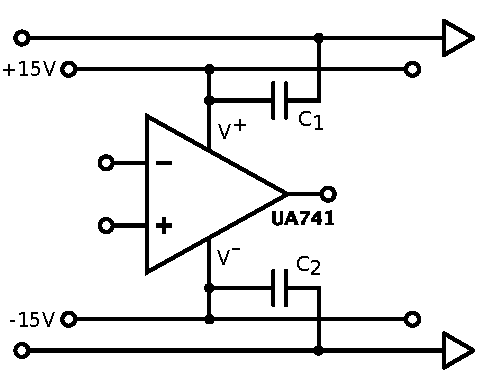
\includegraphics[width=6.5cm]{../E01/latex/alimentazione.pdf}
	\caption{In questo grafico è mostrato lo schema di alimentazione dell'opamp. Le capacità hanno un valore nominale di $C_1=C_2= \SI{100}{\nano\farad}$. La tensione di alimentazione è impostata a $V^+ = \SI{15}{\volt}$ e a $V^- = \SI{-15}{\volt}$ ed è fornita dal generatore di tensione costante.\\
\newline\newline\newline}
 \label{cir1:costante}
\end{SCfigure}

Per quanto riguarda l'alimentazione del circuito, abbiamo collegato i terminali $V^+$ e $V^-$ ad alimentazioni rispettivamente di \SI{+15}{\volt} e \SI{-15}{\volt}. Inoltre, in quanto immersi in un ambiente elettronicamente rumoroso, abbiamo inserito nel circuito due capacitori con lo scopo di evitare problemi di noise elettronico.
Per maggiore chiarezza di esposizione, questa configurazione sarà nascosta negli schemi successivi, ma comunque presente sulla breadboard.

%\newpage
\subsection{Generatore di corrente}

Come primo circuito abbiamo montato un generatore di corrente costante, ossia un dispositivo in grado di erogare una corrente costante indipendentemente dal carico a cui è collegato.
Poiché il nostro interesse era osservare il comportamento del circuito per diversi valori della resistenza di carico $R_2$, abbiamo utilizzato \textit{trimmer} come resistenza variabile. In Figura \ref{cir1:gen_continua} è riportato lo schema circuitale.
Utilizzeremo ora le \textit{regole d'oro} per risolvere il circuito. B si trova a potenziale di comune, quindi per (\ref{eq1:regola_V}) anche A sarà allo stesso potenziale, che considereremo nullo. Dunque è verificato
\begin{equation}
V_{gen}=I R_1
\label{eq1:gen_1}
\end{equation}

\begin{wrapfigure}[18]{r}{0.52\textwidth}
  \caption{Schema del generatore di corrente costante. Abbiamo utilizzato $R1=3.85 \pm 0.01 \,\si{\kilo\ohm}$ e $V_{gen}=3.85 V$, mentre $R_2$ è variabile. Come amperometro è stato utilizzato il multimetro, mentre sia per alimentare l'opamp sia come generatore di tensione costante, abbiamo utillizzato il generatore DC Agilent E3631A.}
  \begin{center}
    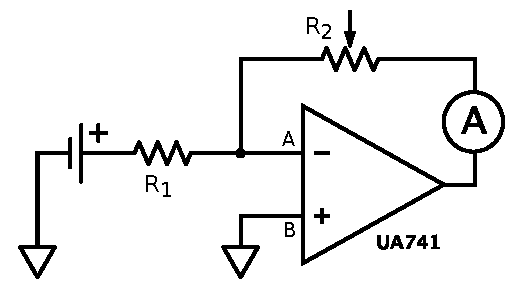
\includegraphics[width=0.42\textwidth]{../E01/latex/c1.pdf}
  \end{center}
\label{cir1:gen_continua}
\end{wrapfigure}

Per la legge di Kirkhhoff sui nodi e dalla eq. (\ref{eq1:regola_I}), si ottiene che la corrente passante per la resistenza di carico è uguale alla corrente $I$, definita dall'eq. (\ref{eq1:gen_1}).

Come possiamo osservare, l'intensità di corrente passante per la resistenza $R_2$ è indipendente dal valore della resistenza stessa. Infatti la tensione di output dell'opamp verrà da esso stesso modificata in modo da far passare sempre lo stesso valore di corrente attraverso il carico.
Ciò avviene grazie al fenomeno di \textit{negative feedback}, o retroazione negativa, che permette all'opamp di controllare la tensione di output in modo tale da verificare l'eq. (\ref{eq1:regola_V}).
Conoscendo la corrente attraversante $R_2$, possiamo inoltre ricavare il valore di tensione in uscita:

$$V_{out}=-\frac{R_2}{R_1} V_{gen}$$

Per quanto riguarda le misure da noi ricavate, abbiamo deciso di misurare la corrente $I$ passante per la resistenza piuttosto che la tensione di uscita, ponendo un amperometro fra l'uscita dell'opamp e la resistenza di carico $R_2$.
Abbiamo scelto di progettare il circuito affinché fornisse \SI{1}{\milli\ampere}, in modo da rimanere nel range di funzionamento ideale dell'opamp (\SIrange{10}{20}{\milli\ampere}).
Avendo a disposizione una resistenza $R_1=3.85 \pm 0.01\,\si{\kilo\ohm}$, per (\ref{eq1:gen_1}), abbiamo utilizzato una tensione continua di $3.85 V$. A seguire sono riportati i valori sperimentali da noi ricavati (gli errori sono sottointesi essere unitari sull'ultima cifra significativa).

\begin{table}[H]
\center
\caption{Dati da noi registrati con relativi errori.}
{\renewcommand{\arraystretch}{1.4}%
\begin{tabular}{c|c|c|c|c|c|c|c|c}
$R_2$ [\si{\ohm}] & 0.54 & 35.1 & 412 & 1021 & 1996 & 3068 & 4170 & 4719 \\ 
\hline 
$I$ [\si{\milli\ampere}] & 1.002 & 1.002 & 1.002 & 1.002 & 1.002 & 1.002 & 1.002 & 1.002 \\ 
\end{tabular}}
\end{table}


È evidente che il circuito da noi creato fornisce un valore di corrente indipendente dal carico ad esso collegato, quantomeno nel range da noi testato.

\subsection{Sommatore Pesato}

Il secondo circuito che abbiamo preso in esame è un sommatore pesato: nel nostro caso il circuito aquisiva due segnali in ingresso e produceva in uscita un unico segnale ottenuto dalla somma pesata dei due ingressi. In particolare si osserva che il peso di ciascun segnale è dato dal rapporto tra la resistenza di feedback $R_f$ e la resistenza associata al canale di ingresso, $R_1$ e $R_2$. In Figura \ref{cir1:sommatore_pesato} è riportato lo schema del circuito.

\begin{wrapfigure}[21]{l}{0.55\textwidth}
  \begin{center}
    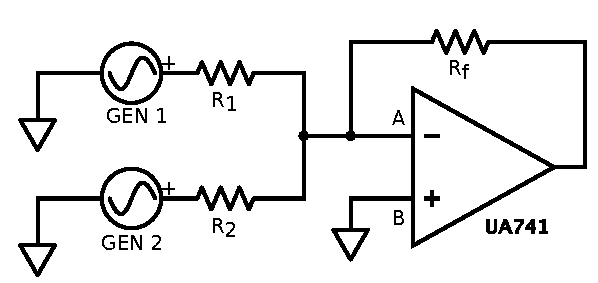
\includegraphics[width=0.40\textwidth]{../E01/latex/c2.pdf}
  \end{center}
  \caption{Schema del sommatore pesato. Come valori abbiamo utilizzato $R_f \approx R_1=(99.9 \pm 0.1)\,\si{\kilo\ohm}$ e $R_2=(49.8 \pm 0.1)\,\si{\kilo\ohm}$, dove per $R_2$ è stato necessario utilizzare un parallelo di due resistenze da \SI{100}{\kilo\ohm}. Come GEN 1 abbiamo utilizzato l'oscilloscopio, mentre per GEN 2 il generatore di forme d'onda. Infine, per valutare la tensione in uscita abbiamo utilizzato l'oscilloscopio.}
\label{cir1:sommatore_pesato}
\end{wrapfigure}

Per risolvere il circuito utilizziamo ancora una volta le \textit{regole d'oro} e le leggi di Kirchhoff. Definendo le tensioni dei generatori 1 e 2 relativamente $V_1$ e $V_2$, si ricavano le seguenti equazioni:
$$V_1 - V_A =I_1 R_1 \qquad V_2 - V_A =I_2 R_2$$
$$V_A - V_{out} =(I_1+I_2) R_f$$
Essendo però B connesso al potenziale di comune, da (\ref{eq1:regola_V}) si ottiene che $V_A = V_B = 0$ che sostituita nelle equazioni precedenti porta a:
\begin{equation}
V_{out}=-R_f \left( \frac{V_1}{R_1}+\frac{V_2}{R_2}\right)
\label{eq1:sum_v_out}
\end{equation}

Analizzando il caso generale di sommatore a cui sono connessi \textit{n} canali in ingresso si può riscrivere la formula (\ref{eq1:sum_v_out}) più elegantemente. Definendo il peso relativo di ogni segnale come $\phi_i = \frac{R_f}{R_i}$:
\begin{equation*}
V_{out}=-\sum^{n}_{i=1} \frac{R_f}{R_{i}}V_{i}=-\sum^{n}_{i=1} \phi_i V_{i}
\end{equation*}

Noi abbiamo optato per valori semplici dei pesi: $\phi_1=1$ e $\phi_2=2$. Per ottenere questi valori abbiamo utilizzato i seguenti valori di resistenza: $R_f=R_1=\SI{100}{\kilo\ohm}$ e $R_2=\SI{50}{\kilo\ohm}$.
Presentiamo ora i grafici di alcune forme d'onda in uscita.

\begin{figure}[ht]
 \centering
   {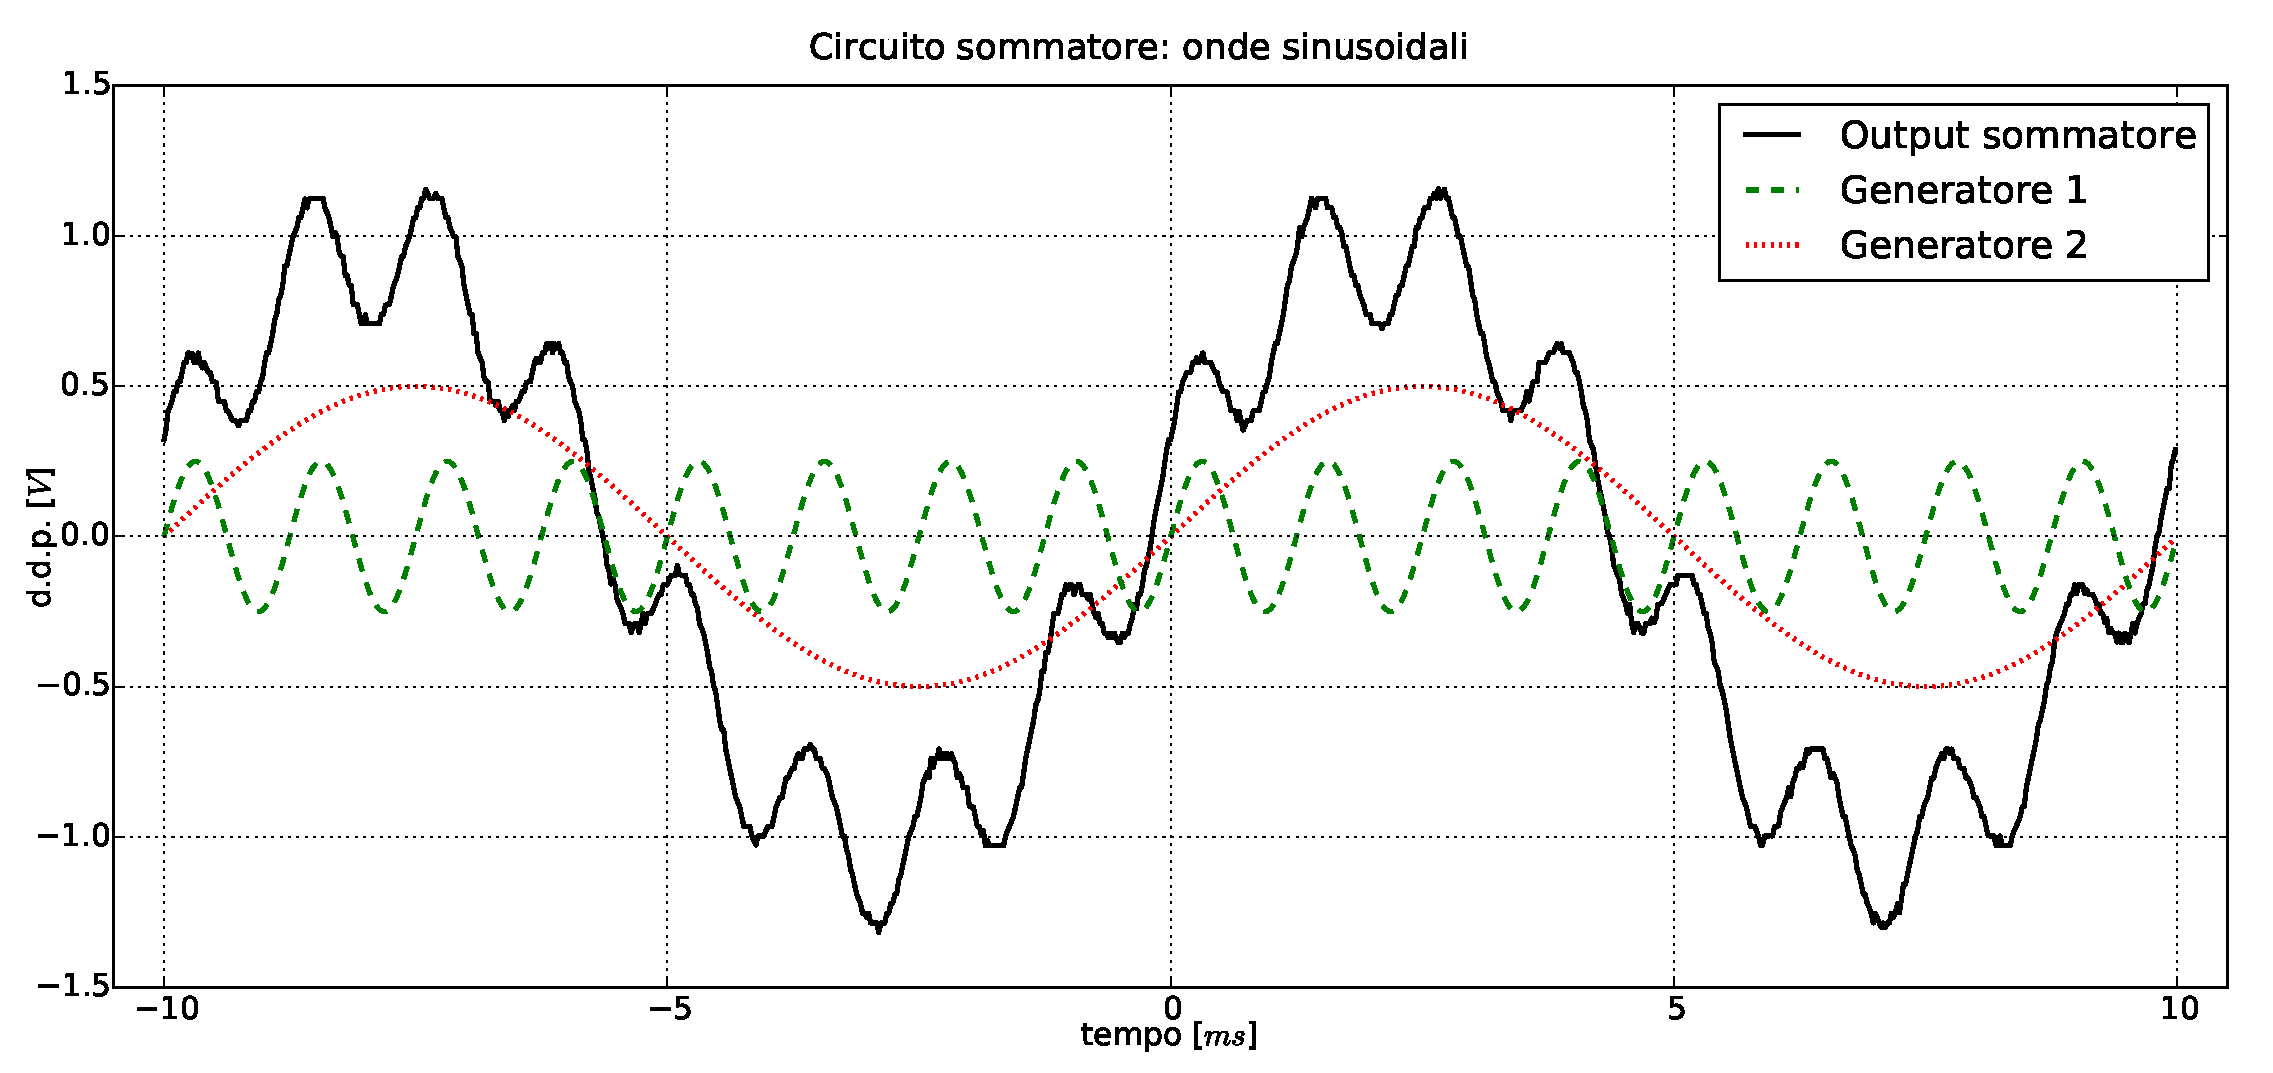
\includegraphics[width=14.8cm]{../E01/latex/sinsin.pdf}}
 \caption{Grafico della tensione in uscita. Il generatore 1 (generatore dell'oscilloscopio) produce un'onda sinusoidale di $\nu=800$ \si{\hertz} e $V^1_{pp}=500$ \si{\milli\volt}; il generatore 2 (generatore di forme d'onda) produce un'onda sinusoidale di $\nu=100$ \si{\hertz} e $V^2_{pp}=1000$ \si{\milli\volt}. Si può verificare facilmente per l'ampiezza massima che $V_{out} = \phi_1 V^1_{pp}+\phi_2 V^2_{pp}$.}
 \label{gr1:onde1}
\end{figure}

\begin{figure}[ht]
 \centering
   {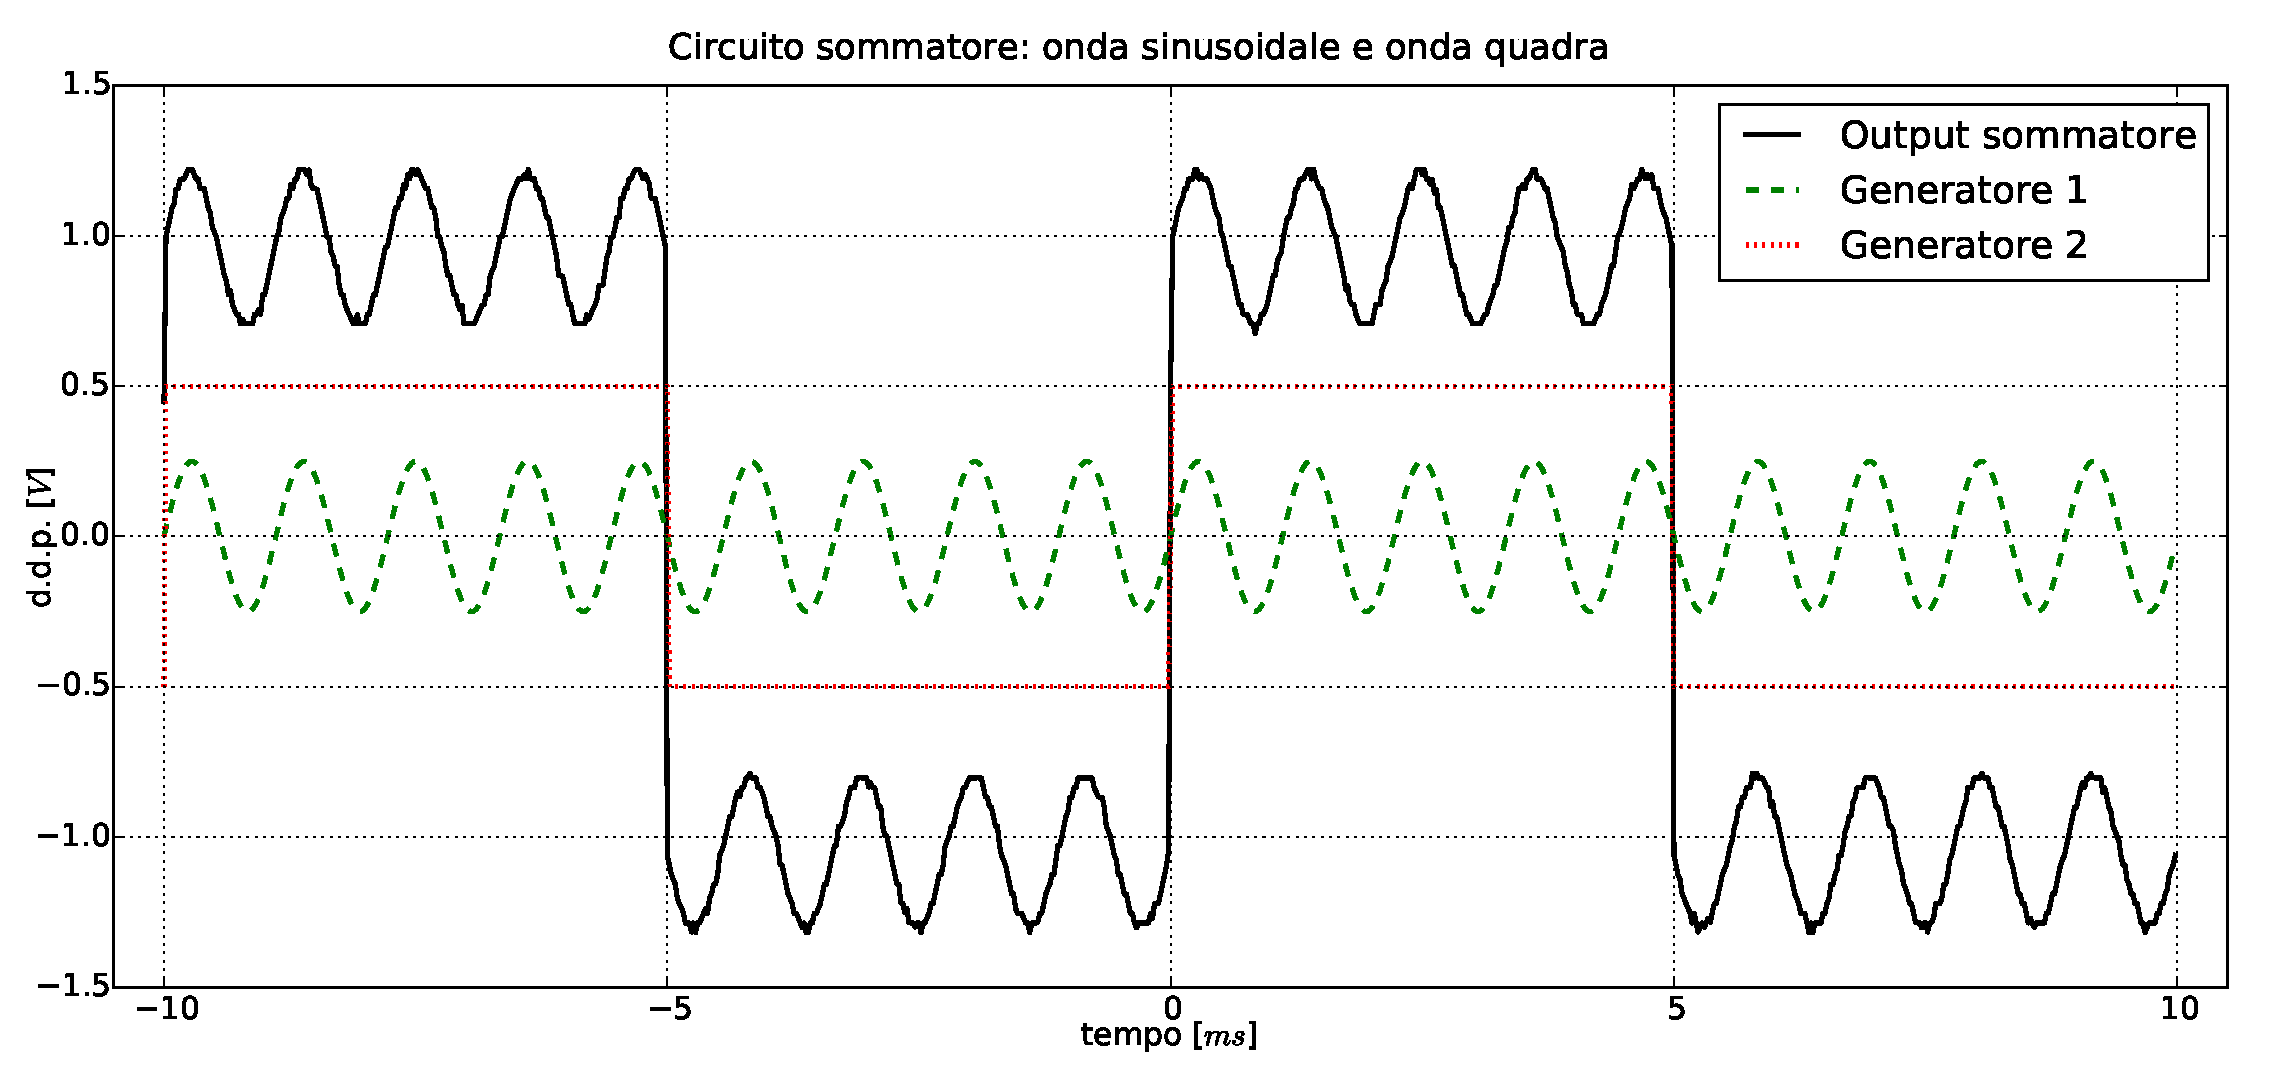
\includegraphics[width=14.8cm]{../E01/latex/sinquad.pdf}}
 \caption{Grafico della tensione di uscita. Il generatore 1 (generatore dell'oscilloscopio) produce un'onda sinusoidale di $\nu=900$ \si{\hertz} e $V^1_{pp}=500$ \si{\milli\volt}; il generatore 2 (generatore di forme d'onda) produce un'onda quadra di $\nu=100$ \si{\hertz} e $V^2_{pp}=1000$ \si{\milli\volt}. Anche in questo caso si può verificare facilmente per l'ampiezza massima che $V_{out} = \phi_1 V^1_{pp}+\phi_2 V^2_{pp}$.}
 \label{gr1:onde2}
\end{figure}

\begin{figure}[ht]
 \centering
   {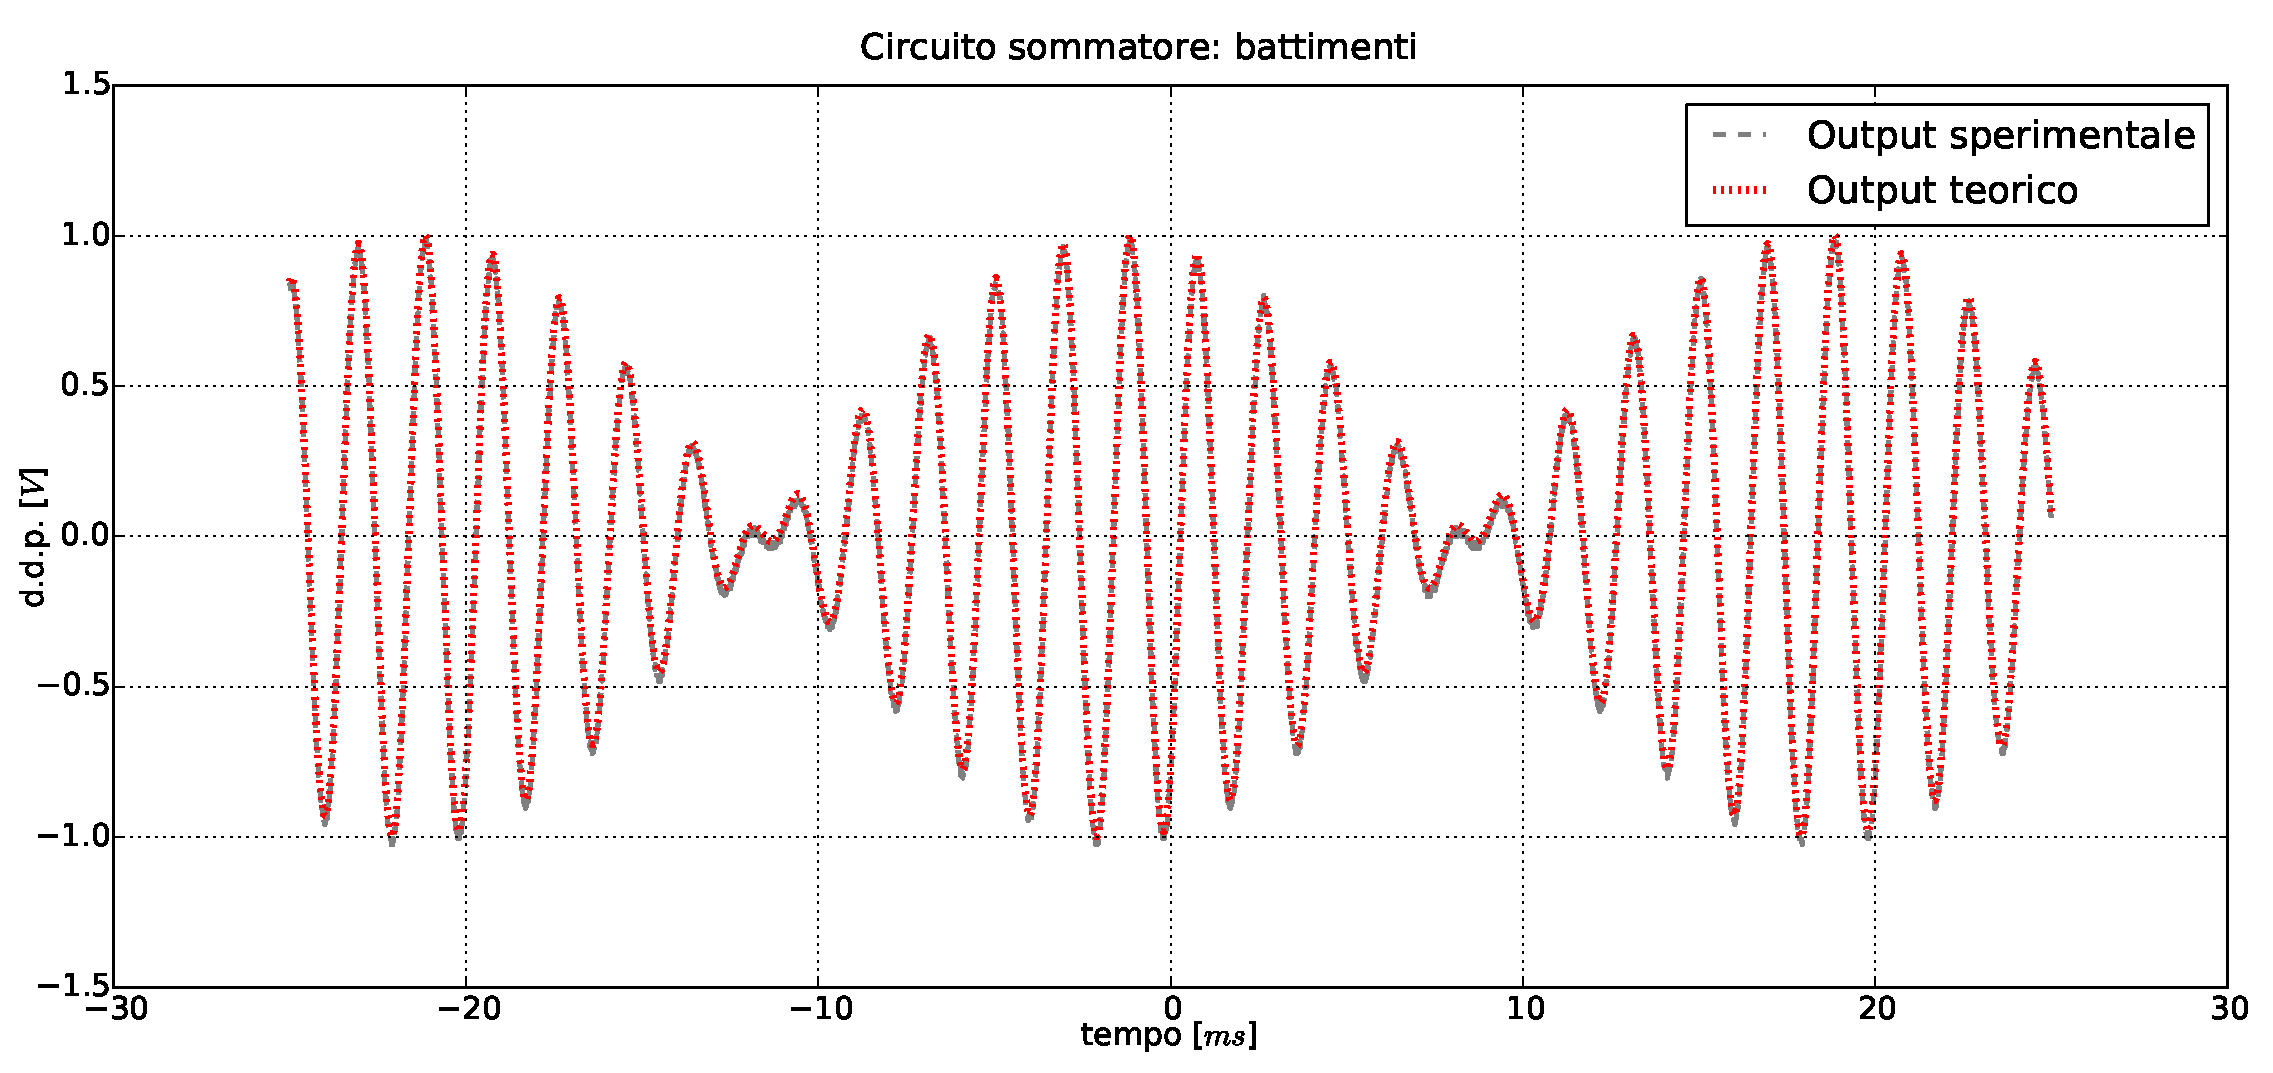
\includegraphics[width=14.8cm]{../E01/latex/battimenti_ideali.pdf}}
 \caption{In questo grafico il generatore 1 (oscilloscopio) produce un'onda sinusoidale di $\nu_1=550$ \si{\hertz} e $V^1_{pp}=1000$ \si{\milli\volt}, mentre il generatore 2 (Agilent 33120A) produce un'onda sinusoidale di $\nu_2=500$ \si{\hertz} e $V^2_{pp}=500$ \si{\milli\volt}. In questa condizione si può notare che la somma di due onde sinusoidali di ugual ampiezza ma con frequenza simile produce un'onda sinusoidale la cui ampiezza è modulata da un coseno secondo la legge $V_{out} = 2Acos\left[\pi(\nu_1 - \nu_2)t\right]sin\left[\pi(\nu_1 + \nu_2)t\right]$. Si può notare che nel grafico in Figura \ref{gr1:onde1} l'effetto dei battimenti non è osservabile poiché le frequenze delle due onde non sono simili} 
 \label{gr1:battimenti}
\end{figure}
